\documentclass[12pt]{standalone}
\usepackage{amsmath, relsize, tikz}
\usepackage{xcolor}
\usepackage{pgffor} % LATEX
\input pgffor.tex % plain TEX
\usetikzlibrary{matrix}
\usetikzlibrary{knots}
\usetikzlibrary{intersections,backgrounds}
\usetikzlibrary{patterns}
\begin{document}
    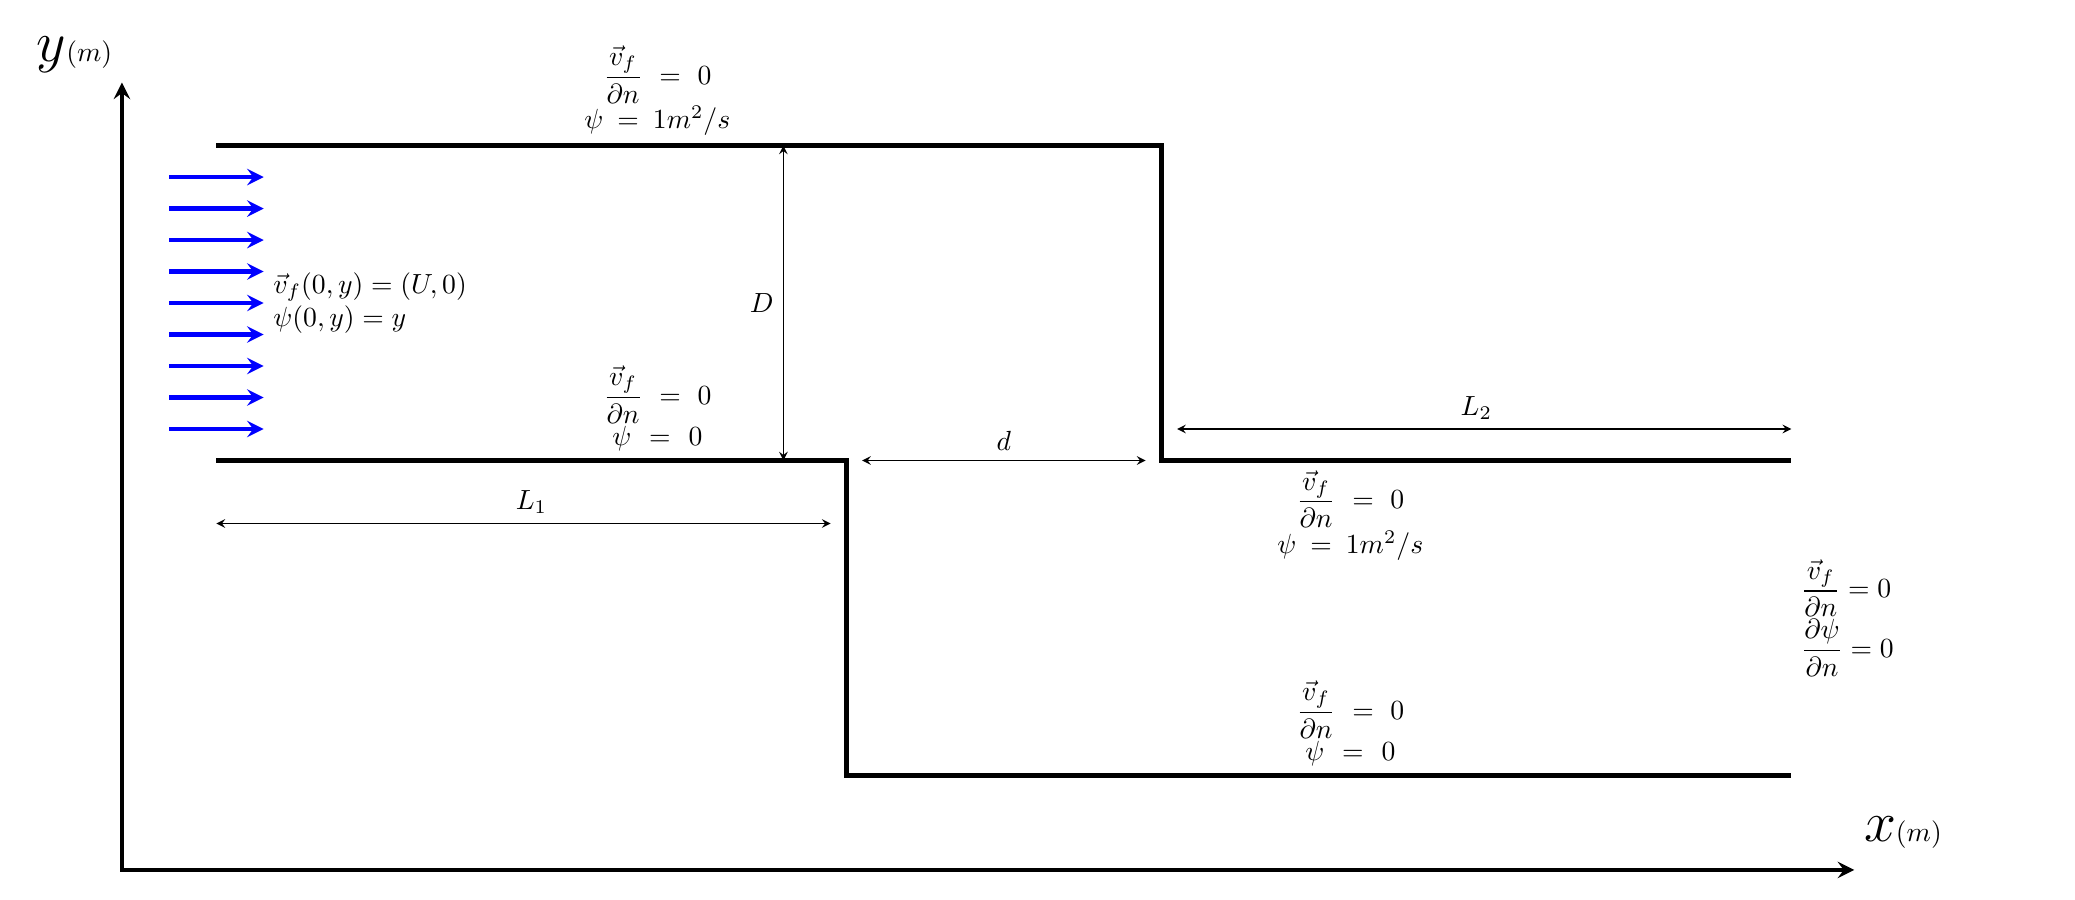
\begin{tikzpicture}[scale=4.0, >=stealth]
        \draw [ultra thick] (0, 2) -- (3, 2) -- (3, 1) -- (5, 1);
        \draw [ultra thick] (0, 1) -- (2, 1) -- (2, 0) -- (5, 0);

        \draw [<->, ultra thick] (-0.3,2.2) -- (-0.3,-0.3) -- (5.2,-0.3);

        \node [above left] at (-0.3, 2.2) {{\huge $y$}{$(m)$}};
        \node [below right] at (5.2, -0.1) {{\huge $x$}{$(m)$}};

        \node [above, text width=3cm, align=center] at (1.4, 2) {$\dfrac{\vec{v}_f}{\partial n} = 0$\\$\psi = 1m^2/s$};
        \node [above, text width=3cm, align=center] at (1.4, 1) {$\dfrac{\vec{v}_f}{\partial n} = 0$\\$\psi = 0$};
        \node [right, text width=3cm] at (0.15, 1.5) {$\vec{v}_f(0,y) = (U,0)$\\$\psi(0,y) = y$};
        \node [right, text width=3cm] at (5, 0.5) {$\dfrac{\vec{v}_f}{\partial n} = 0$\\$\dfrac{\partial \psi}{\partial n} = 0$};

        \node [below, text width=3cm, align=center] at (3.6, 1) {$\dfrac{\vec{v}_f}{\partial n} = 0$\\$\psi = 1m^2/s$};
        \node [above, text width=3cm, align=center] at (3.6, 0) {$\dfrac{\vec{v}_f}{\partial n} = 0$\\$\psi = 0$};

        \draw [<->] (0.0, 0.80) -- (1.95, 0.80);
        \node [above] at (1.0, 0.80) {$L_1$};
        \draw [<->] (3.05, 1.10) -- (5.0, 1.10);
        \node [above] at (4.0, 1.10) {$L_2$};
        \draw [<->] (2.05, 1.0) -- (2.95, 1.0);
        \node [above] at (2.5, 1.0) {$d$};
        \draw [<->] (1.8, 1.0) -- (1.8, 2.0);
        \node [left] at (1.8, 1.5) {$D$};

        \foreach \y in {0.1, 0.2, ..., 0.9}
        {
            \draw [blue, ->, ultra thick] (-0.15, 1+\y) -- (0.15, 1+\y);
        }
    \end{tikzpicture}
\end{document}

